\documentclass[letter]{article}

\usepackage[english]{babel}
\usepackage[utf8]{inputenc}
\usepackage{amsmath}
\usepackage{graphicx}
\usepackage[colorinlistoftodos]{todonotes}
\usepackage{multicol}

 
\newcommand\tab[1][1cm]{\hspace*{#1}}

\vspace{20pt}
\title{\textbf{On-Demand Distributed Computing Workflow for Physics Analysis at the CMS Experiment}}

\author{Diyaselis Delgado López$^{1,2}$ \\ \\ \small $^1$CERN, Geneva, Switzerland \\ \small $^2$University of Puerto Rico, Mayagüez, Puerto Rico}
\date{\today} 

\begin{document}

\maketitle
\vspace{15pt}
\begin{center}
    
\includegraphics[scale=0.1]{rum}
\end{center}
\vspace{30pt} \\

\newline

A thesis submitted in fulfillment of the requirements for the degree of Bachelor of Science in the High Energy Physics Unit of the Department of Physics
\\
\vspace{15pt}

\newline 
This project was performed under the supervision of Dr. Kati Lassila-Perini, from Helsinki Institute of Physics, and Dr. Sudhir Malik, from University of Puerto Rico Mayagüez
\thispagestyle{empty}

\newpage
\begin{abstract}
The CMS experiment is a strong contributor to the CERN Open Data Portal, the CMS Open Data project aims to release real data collected from proton-proton collisions at the LHC to the public. In doing so, it publishes research level data together with environment, software and instructions on how to use it. These data accompanied with their proper analysis can be used scientific research outside the CMS collaboration.
This project takes part in developing and testing simplified examples of open data while providing a connection to analysis preservation and a new reproducible research data analysis platform. The purpose of this work is to improve and build upon the CMS Open Data release, by allowing users to study higher energy 13 TeV collisions from preserved analyses. 
\end{abstract}

\textit{Keywords}: Open Data, analysis preservation, reproducibility, computing, workflows
\thispagestyle{empty}

\newpage

\tableofcontents

\newpage
\section{Introduction}
\tab This thesis arises from the ongoing work with experimental data from proton-proton collisions analyzed from the CMS (Compact Muon Solenoid) \cite{cms} experiment at the Large Hadron Collider (LHC) \cite{lhc}. Here, experimental data is analyzed to study the fundamental structure of particles and to search for evidence of new particle physics. This particular project is based in High Energy Physics analysis for public use in education and scientific research, and involves using frameworks produced for analysis preservation and reproducibility. 

\tab This paper is organized as follows: in Section II we introduce proton-proton collisions, and we briefly describe the CMS detector in section III. In Section IV, we outline and define our preservation and reproducibility platforms. We then review analyses tested towards open experimental data in Section V and present event analysis results in Section VI. Finally, our conclusions are summarized in Section VII.

\subsection{Proton-proton (pp) collisions at LHC}
\tab The LHC is the largest particle accelerator in the world, stationed at CERN \cite{cern}, the European Organization for Nuclear Research, on the French-Swiss border near Geneva. It is located in an underground tunnel 27 km in circumference. The LHC accelerates high-energy particle beams near to the speed of light, before its components collide together at a primary vertex. Each proton-proton collision between constituents is called an event. The particles produced in events are reconstructed in detectors scattered across the LHC, and used to infer the quantum-mechanical process that occurred in the collision. First, the LHC collided protons at a center of mass energy of 7 TeV, upgraded in 2011 to 8 TeV, and it is currently running at 13 TeV.

\subsection{The CMS experiment}
\tab The CMS experiment is a detector placed at one of the pp collision points in the LHC ring. Collision products travel out from the collision point into the detector. CMS can directly detect muons, electrons, photons and hadronic jets. These jets are clusters of charged particles that result from the formation of hadrons from quarks and gluons produced in collisions. The CMS detector is shown in Figure 1. Towards the center of the detector are trackers, which measure particle positions so that their momenta can be calculated. Magnets curve the tracks of charged particles to enable momentum and charge measurements, ideally to identify the particles resulting from the collisions. Outside the trackers is an electromagnetic calorimeter (ECAL), which measure energy deposits from electrons and photons. Further out is the hadronic calorimeters (HCAL), to measure jets of hadrons. At the outside of the detector are the solenoid and the muon chambers. 
\begin{figure}
    \centering
    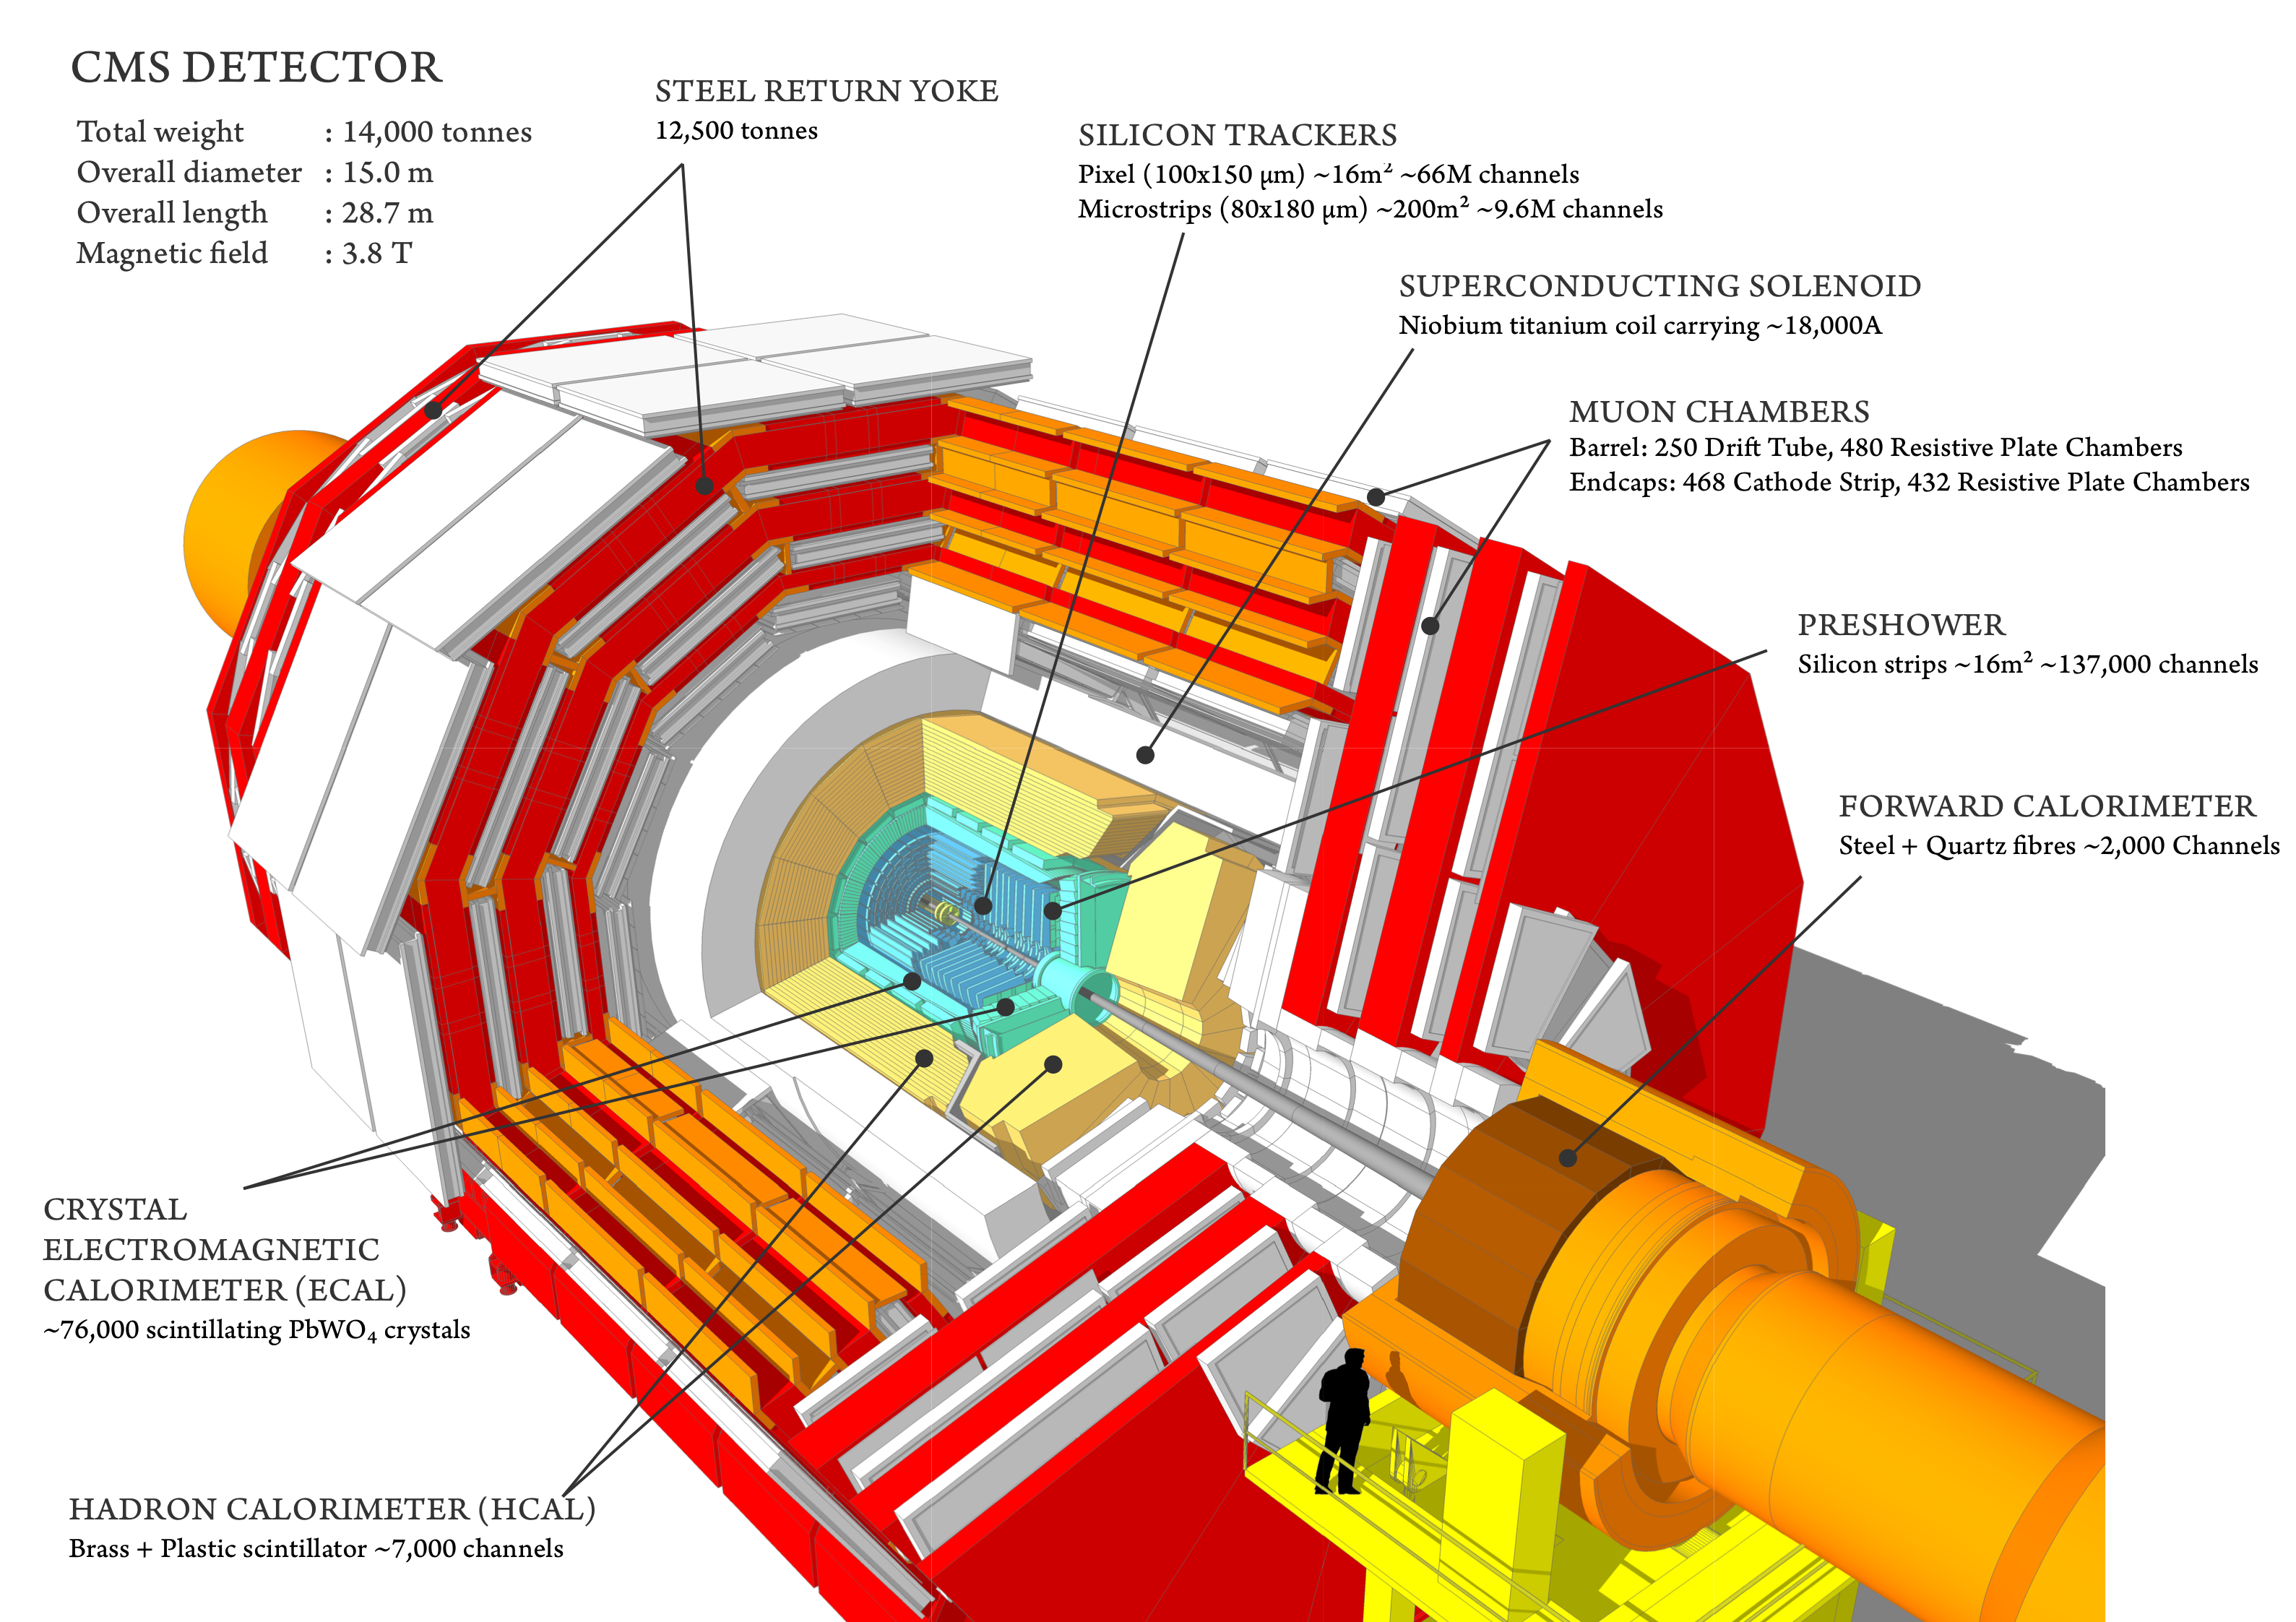
\includegraphics[scale=0.1]{cms}
    \caption{A schematic diagram of a cut-away section of the ATLAS detector. Detector dimensions are shown and people can be seen on site for a sense of scale.}
    \label{fig:cms}
\end{figure}

\section{Analysis preservation and reproducibility platforms}
\tab The CERN Open Data portal (CODP) \cite{codp} is the gateway to an increasing range of data produced at the LHC experiments.
It distributes the preserved product from various research studies, including accompanying software and documentation which is needed to understand and analyze the data being shared.
The CMS experiment releases and distributes through CODP reconstructed data, simulations and software to allow a full scientific
analysis, and provides some simplified data formats for education use. \vspace{5pt}
\\ \tab CMS also provides some analysis examples on the portal. These examples are taken here as use cases for analysis preservation. The analysis record on CODP consists of data (e.g. datasets, code, results) and metadata (e.g. analysis name, contact persons,
publication). This information can then be structured to represent the analysis workflow steps on the CERN Analysis Preservation platform (CAP) \cite{cap}. The CAP service aims to enable physicists to preserve information as it is produced by making it easier to describe, preserve, find, exchange and export information in a fast paced scientific environment. CAP does not require any change in the physicists’ individual arrangements or the terminologies used in the different LHC collaborations. Moreover, this framework is developed to address the need for the long-term preservation of the data analysis process, in order to enable future reproducibility of research
results. \newline
\\ \tab In CAP, information is preserved with the aim of reusing it, for example in ReANA\cite{reana}, a reusable and reproducible research data analysis platform. In ReANA, a preserved analysis can be rerun starting from structured input data, analysis code, containerized environments and computational workflows so that the analysis can be established and run on remote computer clouds.

\section{Physics Analyses on CMS Open Data}
\label{sec:theory}

\subsection{Higgs-to-four-lepton analysis example}
\tab The example studied is a simplified reimplementation of the Higgs discovery using CMS open data inputs, both raw data and Monte-Carlo simulations, from 2011-2012 \cite{higgs}. The data used for the example is actual, meaningful data from the CMS experiment that confirmed the existence of this elusive particle, which then resulted in a Nobel prize. The example contains multiple levels, from very simple to a complete analysis, available with proper CMS software (CMSSW) environment. In order to structure the analysis for ReANA, it must be described under four main categories: inputs, environment, workflow, and code. Taking into consideration the ``Level 3" of the example, an intermediate stage where part of the analysis is runned and the rest is taken from preprocessed data files, we can describe the fabricated output for the discovery of Standard Model Higgs. The method used to create the analysis first entails some theoretical background, then proceeds to make measurements and testing those measurements to compare with established assumptions.\vspace{5pt}
\\ 
\tab According to the Standard Model, one of the ways the Higgs boson can decay is by first creating two Z bosons that then decay further into four leptons (i.e. electrons, muons, etc.). It is not the only process with such a final state, therefore, the analysis sifts through electronic noise, a fundamental quantity for a detector. The theory will not explain in detail the mass of Higgs but it can be obtained from meticulous assumptions; for example, four lepton decay is very dominant in some mass regions and as so it guides this analysis.

\tab The example is worked on the LXPLUS service\cite{lxplus}, lxplus.cern.ch, an interactive logon service to Linux for all CERN users. The cluster LXPLUS consists of public machines provided by the IT Department for interactive work. The example also works with the Open Data virtual machine image  described in the CODP for 2011 and 2012 CMS open data\cite{codpvm}.
Setting up the computing environment implies building a specific software area, in this case, CMSSW\_5\_3\_32. This assures that there is a working ROOT setup and all CMS code framework is at our disposal. Following step is to add analysis code for both the data example and the Higgs simulation example. Finally, we need to capture the analysis workflows, containing the commands we have to run, to obtain the final plot. The ReANA platform captures the analysis workflows and runs the commands remotely to obtain the outputs of any example.\vspace{5pt}
\\
\tab After structuring the analysis and stating any initial conditions, a physicist only needs to create the computational workflows ReANA follows, these include workflows describing: inputs, command steps, and overall schematics. For the Higgs to 4 lepton example, the inputs were listed as so:
\begin{small}
\begin{multicols}{2}
\hspace{14pt}DY1011.root 
\\\tab DY1012.root
\\\tab DY101Jets12.root
\\\tab DY50Mag12.root
\\\tab DY50TuneZ11.root
\\\tab DY50TuneZ12.root
\\\tab DYTo2mu12.root
\\\tab DoubleE11.root
\\\tab DoubleE12.root
\\\tab DoubleMu11.root
\\\tab DoubleMu12.root
\\\tab HZZ11.root
\\\tab HZZ12.root
\\\tab TTBar11.root
\\\tab TTBar12.root
\\\tab TTJets11.root
\\\tab TTJets12.root
\\\tab ZZ2mu2e11.root
\\\tab ZZ2mu2e12.root
\\\tab ZZ4e11.root
\\\tab ZZ4e12.root
\\\tab ZZ4mu11.root
\\\tab ZZ4mu12.root
\\\tab Cert\_190456-208686\_8TeV\_\\\tab 22Jan2013ReReco\_Collisions12\_JSON.txt
\end{multicols} 
\end{small}
\vspace{20pt}
\hspace{-18pt} For all these input datasets, the workflow follows a simple yaml format,$``input.yaml"$, in which yaml is a known data serialization standard for all programming languages\cite{yaml}:
\begin{center}
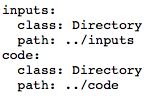
\includegraphics[scale=0.6]{inputs}
\end{center}
Other elements of the analysis called by the $input.yaml$ are the code files used. In this case, to reproduce the Higgs example it was necessary to add the following files: 
BuildFile.xml, HiggsDemoAnalyzerGit.cc, demoanalyzer\_cfg\_level3data.py, demoanalyzer\_cfg\_level3MC.py, M4Lnormdatall\_lvl3.cc.\vspace{5pt}
\\ \tab The analysis will consist of two stages. In the first stage, the original collision data (using demoanalyzer\_cfg\_level3data.py) and simulated data (using demoanalyzer\_cfg\_level3MC.py) will be processed for one Higgs signal candidate with with reduced statistics\cite{github}. For the second stage, the outputs are created, in this case the results are plotted using M4Lnormdatall\_lvl3.cc.
Subsequently, the next workflow describes the commands and steps, mentioned above, to execute the analysis. The format of such workflow is CWL\cite{cwl}, Common Workflow Language, a specification for describing analysis workflows and tools in a way that makes them portable and scalable across a variety of software and hardware environments. The first stage is divided into two workflows, one for raw data and another for Monte-Carlo simulations, named $``step1data.cwl"$, as shown on the left, and $``step1mc.cwl"$, respectively.\\ \\
\hspace{-20pt}
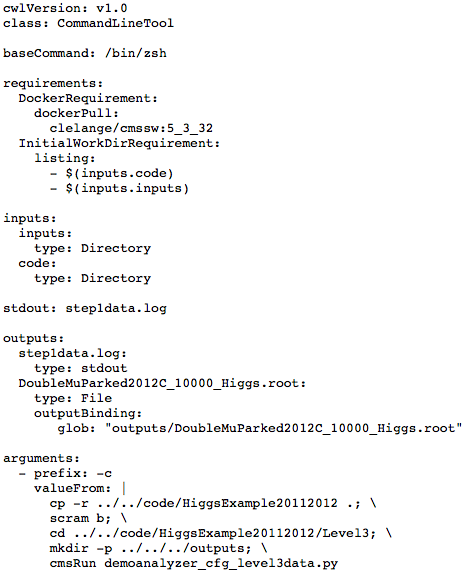
\includegraphics[scale=0.45]{step1data} 
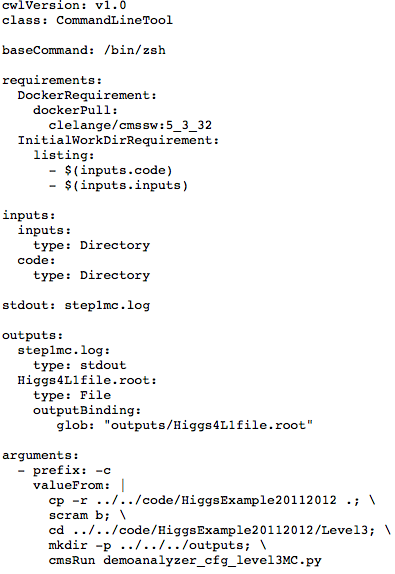
\includegraphics[scale=0.45]{step1mc} \\ \\
\vspace{5pt} The workflow for the second step, $``step2.cwl"$, is:
\begin{center}
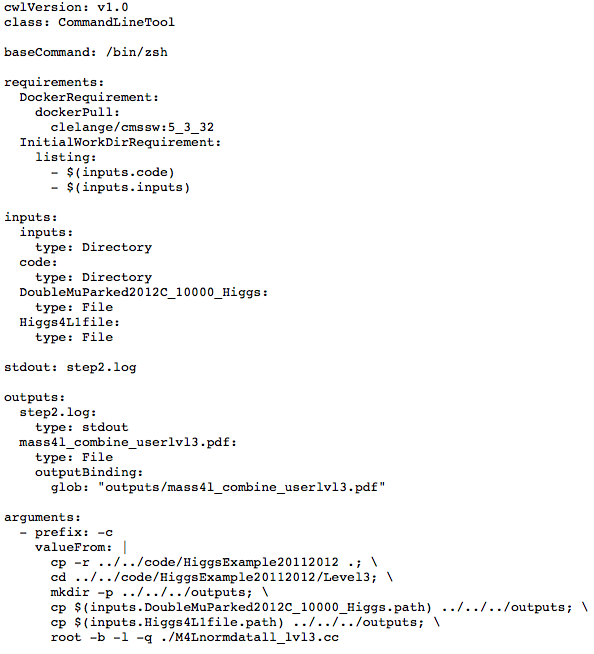
\includegraphics[scale=0.5]{step2}
\end{center}
Finally, the last workflow puts together all the commands and details of the analysis, $``workflow.cwl"$, as displayed below,
\begin{center}
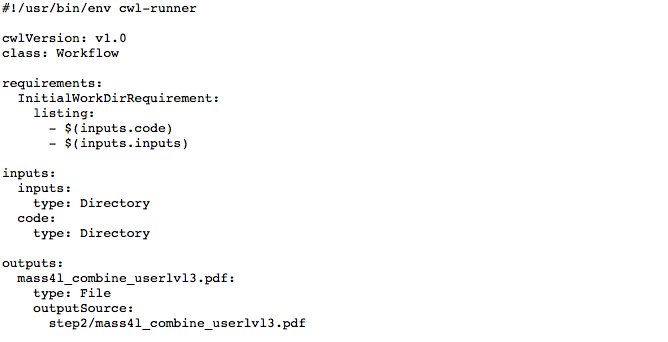
\includegraphics[scale=0.5]{work1}
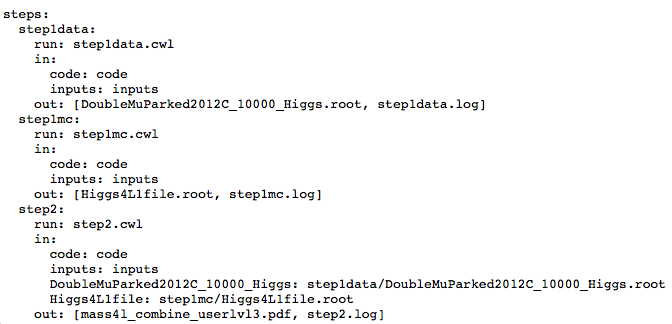
\includegraphics[scale=0.5]{work2}
\end{center}
\tab In order to submit this analysis on the ReANA cloud, a file must be constructed, which recalls the four main characteristics of the analysis (i.e. inputs, code, environment, and workflow), as earlier described. This file follows industry standards and understands simple data formats for an easier implementation from the user. This descriptive file is standardized for every analysis to be run on ReANA, as so it is named $``reana.yaml"$,
\begin{center}
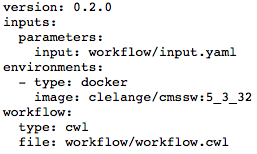
\includegraphics[scale=0.5]{reana}
\end{center}
In the first stage of the Higgs to 4 leptons example on ReANA, the data analysis job will produce a root output file containing one Higgs candidate from the data, and the simulation analysis job a root file containing the Higgs signal distributions with reduced statistics.At the second stage both files are analyzed using root macro and produce the output plot.
\begin{center}
\hspace{-80pt}
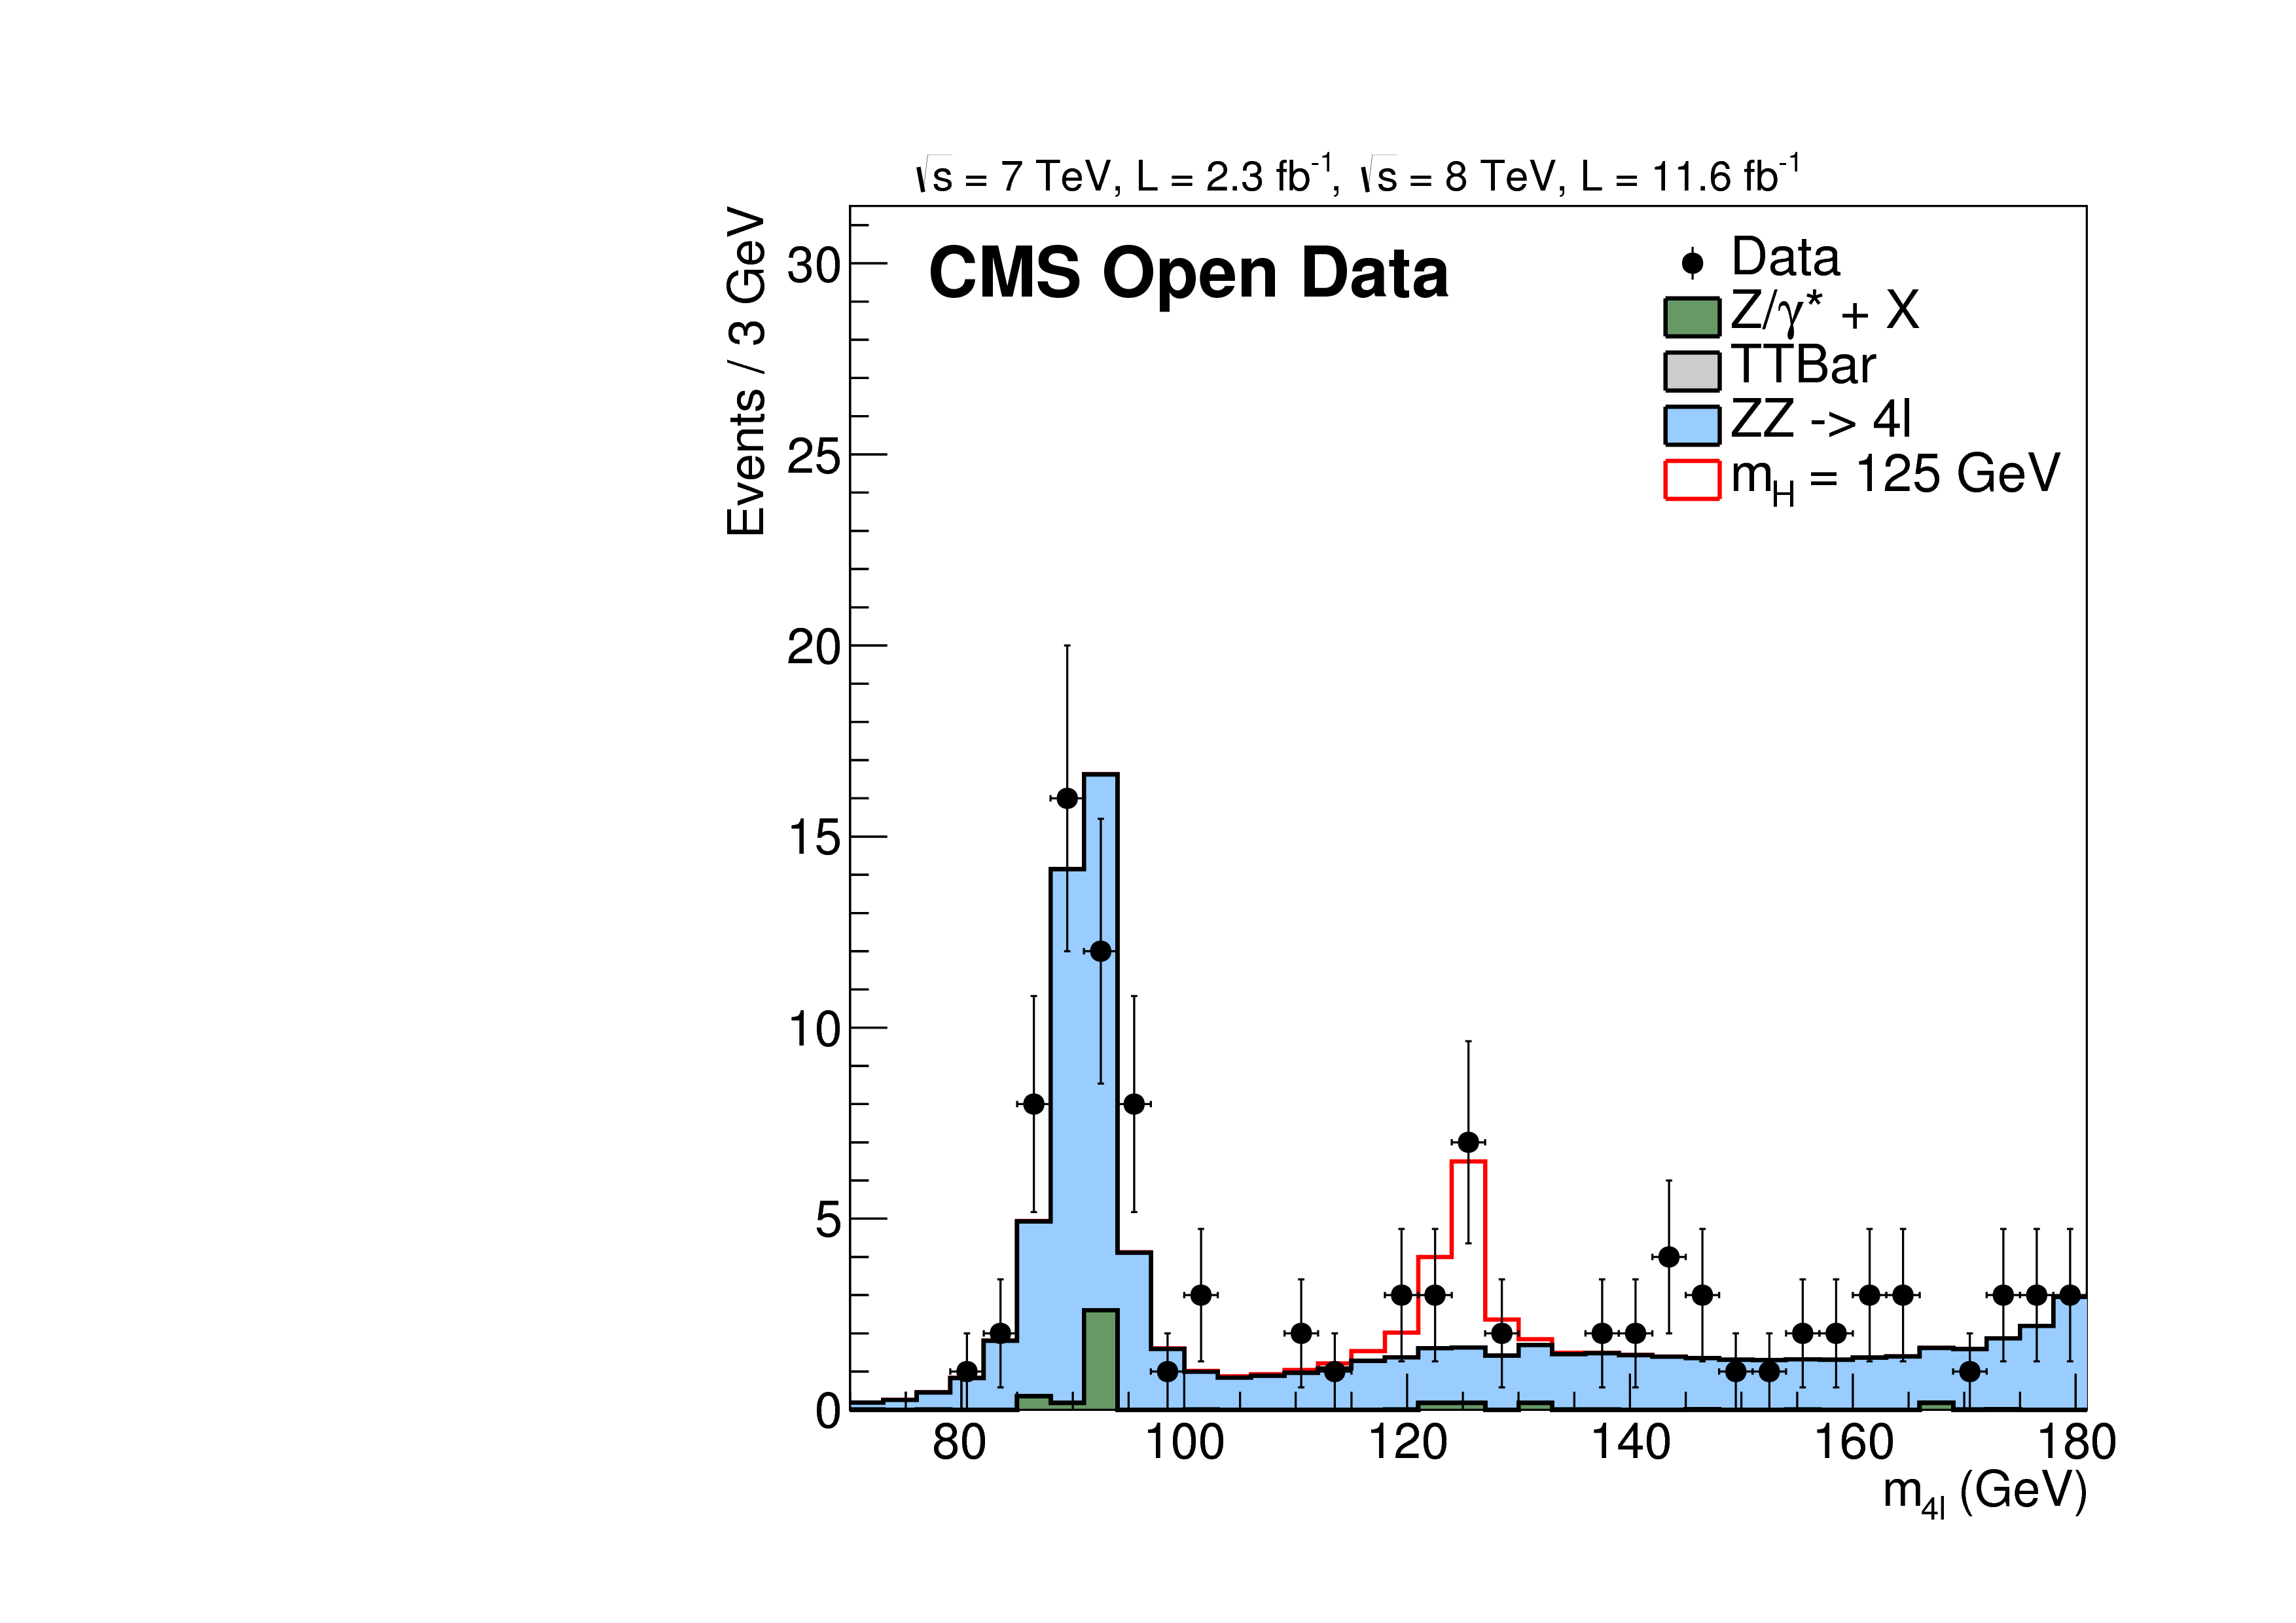
\includegraphics[scale=0.075]{plot}
\vspace{-10pt}
\end{center}

\subsubsection{Running the analysis in the ReANA platform}
\tab An analysis can be made reproducible, i.e. rerunnable, by defining the inputs taken into account, the stages which organize its components, the current compute environment and costumed workflow files. It is implied that the contributor has the code locally in their computer, and has a broad idea of which tools are needed like specific analysis frameworks, custom analysis code, Jupyter notebooks, etc. , and how to run it successfully. Encapsulating the environment involves archiving the type of operating systems, software packages and libraries, CPU and memory resources, among other technicalities. Moreover, the workflow files would describe the steps taken to execute the analysis, if they were simple shell command or complex computational workflows, in order to get expected outcomes such as plots, histograms, and any other files. After structuring the analysis, the research repository should be organized according to inputs, code, environments, and workflows directories. 

Next step is, ideally, to install the reana-client. This process uses the LXPLUS Cluster, lxplus.cern.ch, for which the user simply logs in using their account. 


\subsection{Reprocessing AOD from 2010-2012 RAW samples}
\tab Apart from the previous example, further testing of the preservation and reproducibility platforms is in order, therefore, for the newest data release from the Open Data Portal there is an example that entails the reconstruction of open data and comparison of such. 
This example is a simple comparison to validate the reprocessing step on the Open Data VM (Virtual Machine) by comparing the resulting file, newly rereconstructed from the RAW data samples from 2010 to 2012, and the original AOD available on the Open Data Portal. It loops over different physics objects, such as tracks, electrons, muons, photons, jets, taus and missing etc., and fills histograms with P, pt, eta and phi of these objects. These measurements recall to momentum, transverse momentum, spatial coordinate describing the angle of a particle relative to the beam axis, and polar angle in the transverse plane. The new AOD can be reprocessed from RAW with minor modifications like global tag, input file, commenting out unnecessary steps to the configuration file. 

\subsection{Validation Examples}
\tab In addition to the analysis examples, such as the Higgs to 4 lepton analysis described above, CMS also provides code for validation of the datasets served through the CERN Open Data Portal. The inputs are datasets specific to every example, and the code for the analysis used with the CMS Open Data Virtual Machine environment.  Validation examples prove that a result can be obtained with the legacy or open data tools. For instance, a validation example for 2010 datasets consists of: setting up the CMS environment, compiling and running the analysis, and the workflows written for producing a result (e.g. a comparison plot for the dimuon mass spectrum). The ReANA setup described above allows to rerun CMS Open Data
analyses and in doing so it confirms that instructions are correct and runs large-scale analyses relatively fast.

\section{Conclusions}
\tab In this work, CMS analysis examples from CERN Open Data Portal are taken as examples to connect the three data preservation services, CODP, CAP and ReANA.
The preservation of these physics analysis examples ensures that the complete information is structured and reproducible. Workflow steps for the examples were tested locally and on a remote server, proving to be successful in producing the expected outputs. In ReANA, access to the experimental datasets, analysis software area, operating system environment and computational workflow steps remains to be tested. Overall, the implementation of preservation and reproducibility through the CERN Analysis Preservation and ReANA looks promising as more examples continue to be evaluated. 


\begin{thebibliography}{9}
\begin{small}
\bibitem{cms}
\bibitem{lhc}
\bibitem{cern}
\bibitem{codp}
CERN Open Data Portal. 2018, http://opendata.cern.ch. Accessed 2 Aug 2018.
\bibitem{cap}
CERN Analysis Preservation Portal. 2018, https://analysispreservation.cern.ch. Accessed 5 Aug 2018.
\bibitem{reana}
ReANA: Reusable Analyses. 2018, http://www.reana.io/. Accessed 30 Jul 2018.
\bibitem{higgs}
Jomhari, Nur Zulaiha; Geiser, Achim; Bin Anuar, Afiq Aizuddin. 2017,``Higgs-to-four-lepton analysis example using 2011-2012 data". CERN Open Data Portal. DOI:10.7483/OPENDATA.CMS.JKB8.RR42. Accessed 30 Jul 2018.
\bibitem{lxplus}
CERN IT Department. LXPLUS Service. 2013, http://information-technology.web.cern.ch/services/lxplus-service. Accessed 18 Sep 2018.
\bibitem{codpvm}
CMS Collaboration. ``CMS VM Image, for 2011 and 2012 CMS open data". 2014, http://opendata.cern.ch/record/252. Accessed 25 Sep 2018.
\bibitem{yaml}
YAML Ain't Markup Language. 2018, http://yaml.org. Accessed 18 Sep 2018.
\bibitem{github}
``reanahub/reana-demo-cms-h4l". Github, 2018, https://github.com/reanahub/reana-demo-cms-h4l. Accessed 3 Aug 2018.
\bibitem{cwl}
Common Workflow Language. 2018, https://www.commonwl.org/. Accessed 21 Aug 2018.
\end{small}
\end{thebibliography}
\end{document}